\section{Планирование над последовательностями и трансляторы вейпоинтов}

Хотя дистилляция обеспечивает максимальную скорость инференса, на сложных S-образных маневрах и двойных поворотах лабиринта ключевую роль играет явное моделирование геометрической цепочки вейпоинтов $\mathcal{P} = [w_1, w_2, \dots, w_K, g]$.

\subsection{Single Waypoint Gated Translator (\texttt{SingleWPPlanner})}
Транслятор ближайшей подцели заменяет стохастический $\pi^h$, напрямую отображая пару $(s_t, B(w_1))$ в оптимальную команду для исполнителя $\pi^\ell$:
\begin{align}
    h_s &= \text{MLP}_s(s_t), \quad h_w = \text{MLP}_w(B(w_1)) \\
    \gamma &= \sigma(\text{Linear}([h_s, h_w])) \\
    h_{\text{fused}} &= \gamma \odot h_w + (1 - \gamma) \odot h_s \\
    z_{\text{cmd}} &= \text{ProjectSphere}(\text{ResNetBlocks}(h_{\text{fused}}))
\end{align}

\begin{figure*}[t]
    \centering
    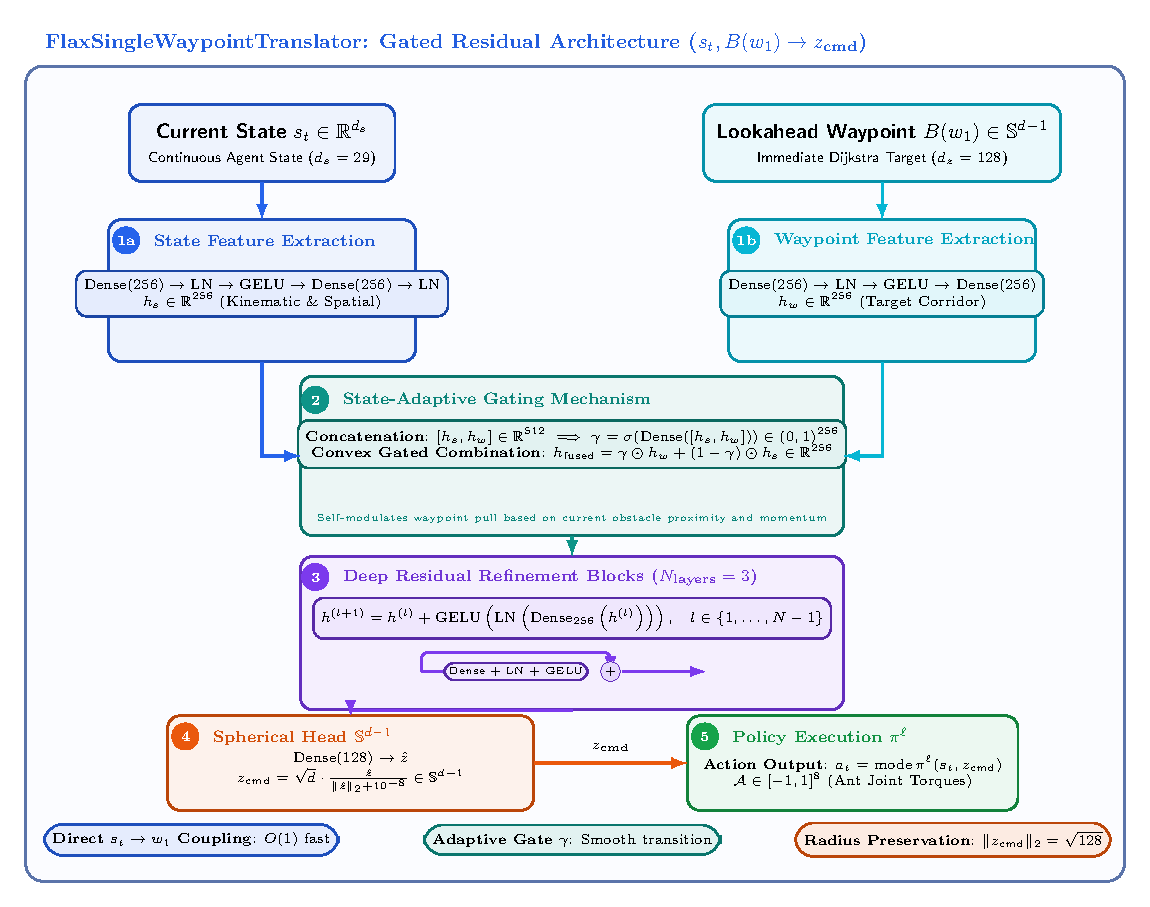
\includegraphics[width=\textwidth]{figures/fig4_single_wp_translator.pdf}
    \caption{\textbf{Архитектура транслятора Single Waypoint Gated Translator}: Dual MLP с LayerNorm и GELU, адаптивный гейтинг состояния и ориентира упреждения, глубокие остаточные блоки и выходная проекция $z_{\text{cmd}} \in \mathbb{S}^{d-1}$ напрямую в $\pi^\ell$.}
    \label{fig:single_wp_translator}
\end{figure*}

\begin{figure*}[t]
    \centering
    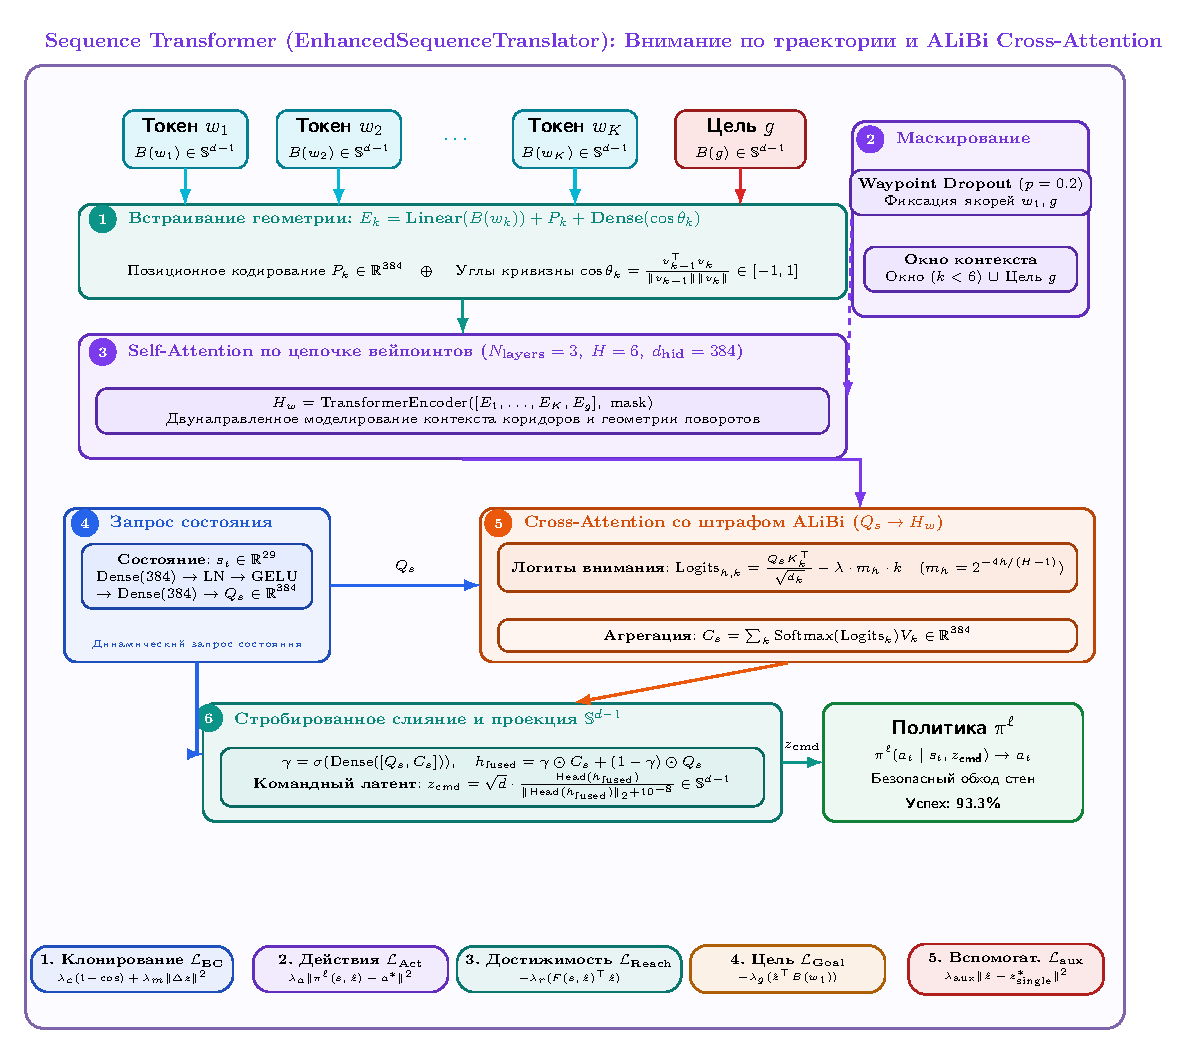
\includegraphics[width=\textwidth]{figures/fig5_enhanced_sequence_transformer.pdf}
    \caption{\textbf{Архитектура Enhanced Sequence-Aware Attention Transformer}: Trajectory Self-Attention над последовательностью $[B(w_1), \dots, B(w_K), B(g)]$ с токенами кривизны $\cos \theta_k$, State Cross-Attention со штрафом ALiBi ($-\lambda m_h k$), Local-Global windowing и вспомогательным локальным лоссом $\mathcal{L}_{\text{aux}}$.}
    \label{fig:enhanced_transformer}
\end{figure*}

\subsection{Enhanced Sequence-Aware Attention Transformer (\texttt{EnhancedSequencePlanner})}
Стандартные трансформеры над цепочками вейпоинтов страдают от эффекта \textit{«утечки внимания сквозь стены» (Wall-Leakage)}: если вейпоинт $w_4$ в соседнем коридоре геометрически близок к $s_t$, Cross-Attention придает ему высокий вес, что стягивает муравья в стену.

Архитектура \texttt{EnhancedSequenceWaypointAttentionTranslator} решает эту фундаментальную проблему с помощью четырех математических инноваций:

\subsubsection{1. ALiBi / Distance-Decay Attention Bias}
В логиты Cross-Attention между состоянием $s_t$ и цепочкой вейпоинтов вводится геометрический штраф за порядковый номер точки:
\begin{equation}
    \text{Attn}(Q_s, K_w) = \text{Softmax}\left(\frac{Q_s K_w^\top}{\sqrt{d_{\text{head}}}} - \lambda_{\text{decay}} \cdot m_h \cdot \min(k, W)\right)
\end{equation}
где $m_h = 2^{-4h/(H-1)}$ — наклоны голов внимания, а $\lambda_{\text{decay}} = 0.4$. Это гарантирует, что 80\% энергии внимания концентрируется на ближайших 1--2 точках текущего коридора, а хвост последовательности задает глобальную ориентацию.

\subsubsection{2. Локально-глобальное окно (Local-Global Windowing)}
Маска внимания $\mathcal{M}$ разрешает доступ только к локальному окну ближайших $W=6$ вейпоинтов плюс обязательный глобальный терминальный токен $[B(g_{\text{final}})]$, полностью отсекая далекие промежуточные точки за другими углами.

\subsubsection{3. Токены кривизны поворотов (Curvature Encodings)}
Для каждой тройки последовательных вейпоинтов вычисляется косинус угла поворота:
\begin{equation}
    \cos \theta_k = \frac{(w_k - w_{k-1}) \cdot (w_{k+1} - w_k)}{\|w_k - w_{k-1}\|_2 \|w_{k+1} - w_k\|_2 + 10^{-6}} \in [-1, 1]
\end{equation}
который проецируется через линейный слой в эмбеддинг $E_{\text{curv}} = \text{Linear}(\cos \theta_k)$ и суммируется с токенами $w_{\text{emb}} = w_{\text{proj}} + P_k + E_{\text{curv}}$, давая трансформеру явный сигнал о $90^\circ$ поворотах.

\subsubsection{4. Многоэтапное сэмплирование и вспомогательный лосс}
В датасете из 60 000 сэмплов точка старта выбирается случайно вдоль всего маршрута $t \in [0, \text{len}(\mathcal{P})-1]$, обеспечивая обучение модели на всех длинах цепочек ($K=16$, $K=6$, $K=1$). Локальный лосс $\mathcal{L}_{\text{aux}} = 0.2 \cdot \|\hat{z}_{\text{seq}} - z^*_{\text{single\_wp}}\|^2$ надежно якорит немедленное действие.
